%
% File:    thesis.tex
%
% Version: 1.00
% Date:    ?
%
% Description:
%   Top level file for the dissertation or thesis.
%   Includes preamble, chapters and appendices from separate files.
%

%%%%%%%%%%%%%%%%%%%%%%%%%%%%%%%%%%%%%%%%%%%%%%%%%%%%%%%%%%%%%%%%%%%%%%%%%%%%%%%
%
% Masters Proposal.tex
%
%                       Catherine Honegger (16 January 2017)
%
%
%
%%%%%%%%%%%%%%%%%%%%%%%%%%%%%%%%%%%%%%%%%%%%%%%%%%%%%%%%%%%%%%%%%%%%%%%%%%%%%%%%

%\documentclass[10pt,twocolumn]{witseiepaper}
\documentclass[MScDiss,altheaders,colorlinks,a4paper]{wits-eie-thesis}
\usepackage{useful-packages} % There are lots of useful packages and command shortcuts here. Review and uncomment what you need.
% in-document links, bibliographic citations, urls
\linkcolors{Black}{Black}{Black}

% title page and PDF document properties

%\usepackage{KJN}
\usepackage[margin=1in]{geometry}
\usepackage{graphics}
%\usepackage[top=30mm, bottom=30mm, left=40mm, right=30mm]{geometry}
%
% PDF Info
%
\ifpdf
\pdfinfo{
/Title (Masters Proposal)
/Author (Catherine A Honegger)
/CreationDate (D:201701161221)
/ModDate (D:201701161221)
/Subject (Masters Proposal)
/Keywords (Masters Proposal)
}
\fi

%%%%%%%%%%%%%%%%%%%%%%%%%%%%%%%%%%%%%%%%%%%%%%%%%%%%%%%%%%%%%%%%%%%%%%%%%%%%%%%
\begin{document}
	
%%%%%%%%%%%%%%%%%%%%%%%%%%%%%%%%%%%%%%%%%%%%%%%%%%%%%%%%%%%%%%%%%%%%%%%%%%%%%%%
\begin{titlepage}
	\setcounter{page}{0}  % fix for hyperref issue
	\hyphenpenalty=10000
	\vspace*{50pt}
	\pdfbookmark[1]{THE EXTENDIBILITY OF MULTI-DIMENSIONAL SPARSE ARRAY REPRESENTATIONS FOR DATA WAREHOUSING}{TitlePage}
	{\Large \bfseries \raggedright THE EXTENDIBILITY OF MULTI-DIMENSIONAL SPARSE ARRAY REPRESENTATIONS FOR DATA WAREHOUSING\par} 
	\vspace*{40pt}
	\pretolerance=100{\Large \bfseries Catherine Ann Honegger \par}
	\vspace*{\fill}{\large \scshape \centering \eeThDraft \par}
	\vspace{\fill}
	\ifx\@putlogo\@putlogotrue
	{
		% no logo on title page
		\begin{center}\end{center}
	}
	\fi
	\hyphenpenalty=1000
	\vspace{\fill}
	{
		A %dissertation
		masters proposal submitted to the Faculty of Engineering and the Built Environment, University of the Witwatersrand, Johannesburg, in fulfilment of the requirements for the degree of Master of Science in Engineering.\par
		\vspace*{2em}
		Johannesburg, September\space2017
		
		\vspace*{1em}
		\normalsize
		\textit {The financial assistance of the National Research Foundation (NRF) towards this research is hereby acknowledged. Opinions expressed and conclusions arrived at, are those of the author and are not necessarily to be attributed to the NRF.}
	}
	\hyphenpenalty=1000
\end{titlepage}
	
%\begin{titlepage}
%	\begin{center}
%		
\includegraphics[width=0.3\textwidth]{Logo}\\
%		\vspace{1.5cm}
%		\LARGE
%		\textbf{EXTENDIBLE MULTI-DIMENSIONAL SPARSE ARRAY REPRESENTATIONS}\\
%		\vspace{0.5cm}
%		\LARGE
%		MSc Research Proposal
%		
%		\vspace{1.5cm}
%		
%		\textbf{Catherine Ann Honegger}\\
%		\Large
%		School of Electrical and Information Engineering\\
%		University of the Witwatersrand\\
%		South Africa
%		
%		
%		\vfill
%		\large
%		A dissertation submitted to the Faculty of Engineering and the Built Environment, University of the Witwatersrand, Johannesburg, in fulfilment of the requirements for the degree of Master of Science in Engineering.
%		
%	
%		
%		\vspace{0.8cm}
%		
%		\large
%		Research Supervisor: Professor Ekow Otoo
%		
%		\vspace{0.8cm}
%		
%		\normalsize
%		Johannesburg, June 2017	
%		
%		\vspace{0.8cm}
%		
%		\normalsize
%		\textit {The financial assistance of the National Research Foundation (NRF) towards this research is hereby acknowledged. Opinions expressed and conclusions arrived at, are those of the author and are not necessarily to be attributed to the NRF.}
%		
%	\end{center}
%\end{titlepage}
%%%%%%%%%%%%%%%%%%%%%%%%%%%%%%%%%%%%%%%%%%%%%%%%%%%%%%%%%%%%%%%%%%%%%%%%%%%%%%%

%\onecolumn
%\section*{DECLARATION}
\pagenumbering{roman}
\clearpage
\phantomsection
%\pagestyle{plain}
\vspace*{50pt}
{ \raggedright \huge \bfseries Declaration \par
	\nobreak
	\vskip 40pt
}
\addcontentsline{toc}{chapter}{Declaration}

I declare that this %dissertation
masters proposal is my own, unaided work, except where otherwise acknowledged. It is being submitted for the degree of Master of Science in Engineering to the University of the Witwatersrand, Johannesburg. It has not been submitted before for any degree or examination to any other University.

\vspace*{\fill} 
{
	\raggedright Signed this \rule{0.8cm}{0.4pt} day of \rule{2.5cm}{0.4pt} 20\rule{0.5cm}{0.4pt} \par \vspace*{2.5cm} % lines lengthened by CRL
	\rule{6cm}{0.4pt}\\
	Catherine A. Honegger \par
	\vspace*{10pt}
}
\newpage

% Preamble - includes the abstract, dedication, and acknowledgements
%!TEX root = main-doc.tex

\begin{preamble}
    %!TEX root = main-doc.tex

\begin{abstract}

Data warehousing is a method used to combine multiple varied datasets into one complete and easily manipulated database as a decision support system. Research over several years has concluded that multidimensional representation of data in data warehousing not only gives a good visual perspective of the data to the user, but also provides a storage scheme for efficient processing. Since data in a data warehouse grows dynamically the multidimensional representation should also be expanded dynamically. Efficient dynamic storage schemes for storing dense, extendible, multidimensional arrays by chunks have been developed in the last couple of years. However in data warehousing the corresponding multidimensional arrays are predominantly sparse arrays. Currently no storage or mapping techniques allow for the extendibility of multidimensional sparse arrays. This research proposes to improve the modelling and representation of extendible multidimensional sparse arrays that involve compression and storage efficiency techniques. Our work addresses extendibility of the sparse array only, and does not concern the shrinking of the sparse array and shows how the techniques are applied in data warehousing.
%150 words - purpose, research methods, procedures employed, major results, conclusions, reccomendations - Start with a statement of the major theme of the dissertation
%1 sentence motivation
%1 sentence done before (related work) relevance, limitation of related works
%Main objective(Main results expected)
%limitation of your work

\end{abstract}

    %%!TEX root = main-doc.tex

\begin{dedication}
\centering
To \ldots
\end{dedication}

    %!TEX root = main-doc.tex

\begin{acknowledgements}
I would like to thank my research supervisor, Professor Ekow Otoo, for taking me on as a masters student. %not only for his excellent guidance during the course of my research work, but also for the ideas he suggested, and his patient revision of my dissertation. 
My special thanks also go to Professor Ken Nixon for his help and support throughout the project.

I am grateful to the University of the Witwatersrand for awarding me a Postgraduate Merit Award as financial assistance during my studies.

I am also grateful to the National Research Foundation (NRF) South Africa for their financial support for my study.
\end{acknowledgements}


    \tableofcontents
    %\listoffigures
    %\listoftables
    %\listofalgorithms
    %\listofsymbols
    %%!TEX root = main-doc.tex

\begin{nomenclature}
    \begin{acronym}[3D] % specify longest acronym to get correct spacing
        \acro{2D}{Two-dimensional}
        \acro{3D}{Three-dimensional}    
    \end{acronym}
\end{nomenclature}

\end{preamble}


% Thesis body - includes introduction, conclusion and all intervening chapters
\pagenumbering{arabic}
%!TEX root = main-doc.tex
%
% File: introduction.tex
%
% Date: ?
%
% Description:
%   Provides an introduction to the thesis and describes the
%   overall structure, chapter-by-chapter.
%
\chapter{Introduction}\label{chap:introduction}
\vspace{-1cm}
\summary{This chapter introduces the research and provides a detailed motivation for the significance of the research.}

%%%%%%%%%%%%%%%%%%%%%%%%%%%%%%%%%%%%%%%%%%%%%%%%%%%%%%%%%%%%%%%%%%%%%%%%%%%%%%%
\section{Problem Motivation}
Over recent years with the increase in smartphone use, internet use, and virtually every activity leaving a digital trace, society has been able to store and collect more data, leading to the emergence of huge databases with quintillion bytes of data being produced everyday \cite{economist:2017:twm}. Data has been dubbed ``The world's most valuable resource'' in 2017 as economists believe it is ``the oil of the digital era'' with the five most valuable listed firms in the world for 2017 being data titans\cite{economist:2017:twm}. 

By combining different data sets, useful information can be retrieved from the stored data. Information resources are incredibly important and valuable in business management and decision-making \cite{golfarelli:2009:dwd,wang:2014sar}. By collecting lots of data, companies are able to improve their products and entice more clients with these improvements \cite{economist:2017:twm}. Due to their significance, these data assets must be stored properly and accessed easily \cite{golfarelli:2009:dwd}. Traditional data analysis tools are not able to handle such growing quantities of data. Thus various applications and technologies for managing big-data and high volume data-streams in data intensive computing is becoming essential. Further big-data, data-mining and machine learning are now of major concern in several scientific domains. Thus the field of “Big Data” research has materialised from the need to store such large quantities of information. Data analysis in all societal domains involves the storage, retrieval, processing and visualisation of huge databases \cite{otoo:2006:esa}. 

Big data is a rapidly growing on a global scale. However there is a bottleneck of technology that is required to extend the capabilities of the field. Several big data technologies are required that currently don't exist, including: architectures, algorithms, and techniques \cite{twala:2017:bda,moukhi:2015:dws}.

%%%%%%%%%%%%%%%%%%%%%%%%%%%%%%%%%%%%%%%%%%%%%%%%%%%%%%%%%%%%%%%%%%%%%%%%%%%%%%%
\section{Significance}
A new phenomenon, known as data warehousing, was developed as a result of the large quantities of data that need to be stored in recent years \cite{golfarelli:2009:dwd}. Data warehousing is a method used to combine multiple varied datasets into one complete and easily manipulated database as a decision support system. On-Line Analytical Processing (OLAP) can then be performed on these databases by an organisation in order to analyse the data, complete data-mining and determine trends. The organisation is then able to build business intelligent decisions by utilising the analysed data. Data warehousing has many applications in medical informatics and public-health, smart cities, mining, energy, physics and financial systems to name a few.

The storage of the datasets influences the accuracy, speed and performance of the data analysis and thus it is crucial to assess how this information is stored and accessed. Research over several years has concluded that multidimensional representation of data in data warehousing not only gives a good visual perspective of the data to the user, but also provides a storage scheme for efficient processing. Several research advancements have been made in multidimensional arrays in order to ensure that the datasets are efficient and inexpensive. Multi-dimensional arrays when used for their selection, aggregation, summation and other range queries are processed more efficiently than their SQL counter part in huge database queries. Since data in a data warehouse grows dynamically the multidimensional representation should also be expanded dynamically. These multidimensional datasets are continuously increasing by appending new data to the dataset as new information is added \cite{otoo:2006:esa}.

Recent breakthroughs in extendible multidimensional arrays have led to a new area of study in data warehousing, which requires further research and development. Efficient dynamic storage schemes for storing dense, extendible, multidimensional arrays by chunks have been developed \cite{nimako:2012:ced,pedereira:2015:cas}. However in data warehousing the corresponding multidimensional arrays are predominantly sparse arrays. It is thus important to analyse extendible multidimensional sparse arrays. There have been a number of advances made in the performance and efficiency of storage schemes for representing multidimensional sparse arrays \cite{otoo:2016:msa,goil:bess,otoo:2014:nas}. However, currently no storage or mapping techniques allow for the extendibility of multidimensional sparse arrays \cite{nimako:2016:cea}. With computation and storage costs being the most expensive part of data warehousing and data-mining, being able to utilize extendible multidimensional sparse arrays will extend the capabilities and domains for big-data analysis. %fix last sentence .....  high efficient processing - minimal mannaer (storage)

%%%%%%%%%%%%%%%%%%%%%%%%%%%%%%%%%%%%%%%%%%%%%%%%%%%%%%%%%%%%%%%%%%%%%%%%%%%%%%%
\section{Problem Statement}
The question raised is whether multidimensional sparse arrays can be stored in such a way that new elements and hyper-plane dimensions can be added. The problem that we are focused on requires the use of new storage techniques to investigate the extendibility of multidimensional sparse arrays with regards to computer performance and storage efficiencies.

An illustrative example of where data warehousing is used is given in Table \ref{tab:example}. Here we will have a fact table displaying the number of items sold on a particular day. This can be further extended into a data repository consisting of items sold per day per store as a relational table. In order to analyse the data to improve a company's sales, they might want to know the number of items sold, or which item is sold more on which day. I.e more carrots are sold on Wednesdays. In order to summarise these values and find patterns in the data roll-in and roll-out queries can be conducted. %drill down summarization of sales per week

\begin{table}[htb]
	\caption{A typical data warehousing example.\label{tab:example}}
	\begin{center}
		\begin{tabular}{p{26mm}cp{35mm}}
			\hline
			&   {\textbf{Item}} & {\textbf{Time}} \\
			&   {\textbf{ Amount}} & \\
			\hline
			Apple   & Monday & 12 \\
			Orange  & Monday & 10\\
			Carrot  & Monday & 9\\
			Banana  & Monday & 9\\
			Grapefruit & Monday & 10\\
			Apple   & Tuesday & 7 \\
			Orange  & Tuesday & 8 \\
			Banana	& Tuesday & 18 \\
			Apple   & Wednesday & 5 \\
			Banana  & Wednesday & 3\\
			Carrot  & Wednesday & 10\\
			\hline
		\end{tabular}
	\end{center}
\end{table}

%%%%%%%%%%%%%%%%%%%%%%%%%%%%%%%%%%%%%%%%%%%%%%%%%%%%%%%%%%%%%%%%%%%%%%%%%%%%%%%
\section{Application}
\textbf{NB - Still working on this section}\\
There are several problems that currently exist in the world that would utilize Big Data. A major example would be the frequency and quality of demographic statistics produced by countries as well as demographic statistics deficits. Such applications are particularly of major demand in developing countries.

\begin{itemize}
	\item There are 46 African countries operating without a complete birth and death registration system.
	\item Population censuses have not been conducted since 2010 in several African countries.
	\item Several African countries have not conducted an agricultural census in the last ten years. South Africa in particular held their last agricultural census in 2007.
\end{itemize}

Having up-to-date, reliable demographic statistics enables people within the population to partake in highly important activities. These include gaining quality education, formal employment, voting in elections, access to financial services, obtaining passports and obtaining IDs to name but a few. Reliable data also enables governments to budget better and improve the delivery of public goods and services \cite{mo:2015:sin}.

%tracking taxes - economic

%%%%%%%%%%%%%%%%%%%%%%%%%%%%%%%%%%%%%%%%%%%%%%%%%%%%%%%%%%%%%%%%%%%%%%%%%%%%%%%
\section{Early Results from Literature}
\textbf{NB - Still working on this section}

%%%%%%%%%%%%%%%%%%%%%%%%%%%%%%%%%%%%%%%%%%%%%%%%%%%%%%%%%%%%%%%%%%%%%%%%%%%%%%%
\section{Contribution to Field}
\textbf{NB - Still working on this section}\\
As data is constantly growing, there needs to be a method to provide for this extendibility. The aim of the proposed study is to improve the modelling and representation of extendible multidimensional sparse arrays so that useful compression and storage efficiency can be determined. The representation of the extendible multidimensional sparse arrays must include the characteristics of an array format, such that the array can take on any designed multiple hyper-plane dimensions. The characteristics of the array allow for easy data access. In addition, this allows for both drill-in and roll-out queries. Where drill-in queries allow for detailed data access and roll-out queries allow for summary data access. %drill down

The modelling of the extendible multidimensional sparse arrays will be able to contribute to developing algorithms that can process data at higher speeds, use less physical computational resources and improve the usage of computational power.
%%%%%%%%%%%%%%%%%%%%%%%%%%%%%%%%%%%%%%%%%%%%%%%%%%%%%%%%%%%%%%%%%%%%%%%%%%%%%%%
%\section{Challenges}
%%%%%%%%%%%%%%%%%%%%%%%%%%%%%%%%%%%%%%%%%%%%%%%%%%%%%%%%%%%%%%%%%%%%%%%%%%%%%%%
%\subsection{"this is not research, this is what any competent engineer knows/can do/can find out."}
%\textit{Conclusion: Currently no storage or mapping techniques for extendible multidimensional sparse arrays exist.}
%\newline
%\newline
%Multidimensional sparse arrays require architectures, algorithms, and techniques that currently don't exist [2].
%\newline
%Architectures, algorithms, and techniques include storage and mapping techniques.
%\newline
%Storage and mapping techniques allow for the extendibility of multidimensional arrays.
%\newline
%Currently no storage or mapping techniques for extendible multidimensional sparse arrays exist.
%%%%%%%%%%%%%%%%%%%%%%%%%%%%%%%%%%%%%%%%%%%%%%%%%%%%%%%%%%%%%%%%%%%%%%%%%%%%%%%
%\subsection{"this is not an important topic to be working on"}
%\textit{Conclusion: Extendible multidimensional sparse arrays are important.}
%\newline
%\newline
%Multidimensional arrays are continuously increasing by appending new data to the dataset as new information is added [1].
%\newline
%In data-warehousing there are often scenarios where sparse arrays occur due to new branches of information being created without any aligned historic data.
%\newline
%Extendible multidimensional sparse arrays are important.

%%%%%%%%%%%%%%%%%%%%%%%%%%%%%%%%%%%%%%%%%%%%%%%%%%%%%%%%%%%%%%%%%%%%%%%%%%%%%%%
\section{Organisation of the Proposal}%%CHANGE TO DISSERTATION IN FUTURE
Chapter \ref{chap:background} provides a background on data warehousing and OLAP, extendible multidimensional dense arrays and multidimensional sparse arrays. Chapter \ref{chap:methodology} provides the proposed methodology for developing extendible multidimensional sparse array representations for data warehousing. The experimental setup is provided in Chapter \ref{chap:experimentalsetup}. Chapter 5 details the preliminary results of the research. Expansion on the preliminary results is discussed in Chapter 6. Possible issues that could arise during the research as well as their proposed solutions are presented in Chapter 7. A schedule for the completion of the research is outlined in Chapter 8. A summary of the proposal is given in Chapter 9. 
%!TEX root = main-doc.tex
%
% File: background.tex
%
% Date: ? 
%
% Description:
%   The background is given to ...
%
%
\chapter{Background} \label{chap:background}

\summary{Give chapter summary}

%%%%%%%%%%%%%%%%%%%%%%%%%%%%%%%%%%%%%%%%%%%%%%%%%%%%%%%%%%%%%%%%%%%%%%%%%%%%%%%%
\section{Data Warehousing}
Information is incredibly important \cite{golfarelli:2009:dwd} 

%%%%%%%%%%%%%%%%%%%%%%%%%%%%%%%%%%%%%%%%%%%%%%%%%%%%%%%%%%%%%%%%%%%%%%%%%%%%%%%%
\section{Early Results}


%%%%%%%%%%%%%%%%%%%%%%%%%%%%%%%%%%%%%%%%%%%%%%%%%%%%%%%%%%%%%%%%%%%%%%%%%%%%%%%%
\section{Result Differentiation}


%%%%%%%%%%%%%%%%%%%%%%%%%%%%%%%%%%%%%%%%%%%%%%%%%%%%%%%%%%%%%%%%%%%%%%%%%%%%%%%%
\section{Methodologies}
In order to develop a model for extendible multi-dimensional sparse arrays, the current representations of extendible multi-dimensional arrays must be analysed. The study of the current representations will give a clear indication of how to integrate the representation of extendible multi-dimensional sparse arrays, so that the model can easily be integrated into the current system, preventing unnecessary additional costs. Once a model has been developed, compression of data as well as computing speed will be assessed.

%%%%%%%%%%%%%%%%%%%%%%%%%%%%%%%%%%%%%%%%%%%%%%%%%%%%%%%%%%%%%%%%%%%%%%%%%%%%%%%%
\section{Sparse Array Representations}
Hairong Wang \cite{wang:2014sar}
\begin{itemize}
	\item Space linear in the number of non-zero elements
	\item Acceleration of operations using General Purpose Computing on Graphics Processing Unit
	\item 2-dimensional arrays
	\begin{itemize}
		\item Compressed Row (or alternatively Column) Storage (CRS/CCS)
	\end{itemize}
	\item multi-dimensional sparse arrays
	\begin{itemize}
		\item Bit-Encoded Sparse Storage (BESS) 
		\item Extended the CRS/CCS known as xCRS and xCCS
		\item PATRICIA Trie Compressed Storage (PTCS)
	\end{itemize}
	\item New storage techniques
	\begin{itemize}
		\item Bit-Encoded Compressed Row (or Column) storage (BxCRS/BxCCS)
		\item Hybrid approach (Hybrid) that combines BESS with xCRS
	\end{itemize}
\end{itemize}
Matrix operations include: 
\begin{itemize}
	\item Get, Insert, Delete, Update
	\item Addition, Multiplication, Subtraction, Division
\end{itemize}
2D sparse array can be represented as a linked list or as triplicate 


%%%%%%%%%%%%%%%%%%%%%%%%%%%%%%%%%%%%%%%%%%%%%%%%%%%%%%%%%%%%%%%%%%%%%%%%%%%%%%%%
\section{Dynamic Sparse Arrays}
Increasing Density
\begin{itemize}
	\item Bounds and structure remain the same
	\item new elements are slot into a chunk where there was a free space
\end{itemize}
Increasing Bound


%%%%%%%%%%%%%%%%%%%%%%%%%%%%%%%%%%%%%%%%%%%%%%%%%%%%%%%%%%%%%%%%%%%%%%%%%%%%%%%%
\section{Big Data Warehouse}
\begin{itemize}
	\item Bill Inmon Defines: A data warehouse is a subject-oriented, non-volatile, integrated, time variant collection of data created for the purpose of management’s decision making.
	\begin{itemize}
		\item A big data solution is a technology and data warehousing is an architecture.
	\end{itemize}
	\item Ralph Kimball defines: A data warehouse is a copy of transaction data specifically structured for query and analysis.
	\item Volume - Scalability, storage to grow - investigate using a parallel file system
	\item Velocity - Cope with speed, rate at which data comes in
	\item Variety - Data types
	\item Veracity - validity
	\item Value
	\item Fault tolerance must be researched
\end{itemize}

%%%%%%%%%%%%%%%%%%%%%%%%%%%%%%%%%%%%%%%%%%%%%%%%%%%%%%%%%%%%%%%%%%%%%%%%%%%%%%%%
\section{Big Data Representations}
\begin{itemize}
	\item Capable of holding very large amounts of data.
	\item Hold the data in inexpensive storage devices.
	\item Processing is done by the “Roman census” method.
	\item Data is stored in an unstructured format.
	\item Hierarchical Data Format (HDF5)
	\begin{itemize}
		\item Data model, library, and file format for storing and managing data
		\item Supports an unlimited variety of datatypes, and is designed for flexible and efficient I/O and for high volume and complex data. 
		\item Portable and extensible, allowing applications to evolve in their use of HDF5.
		\item Tools and applications for managing, manipulating, viewing, and analyzing data in the HDF5 format. 
		\item Organized in a hierarchical structure, with two primary structures: groups and datasets. 
		\begin{itemize}
			\item group: a grouping structure containing instances of zero or more groups or datasets, together with supporting metadata. 
			\item dataset: a multidimensional array of data elements, together with supporting metadata. 
		\end{itemize}
	\end{itemize}
	\item Hadoop
	\begin{itemize}
		\item Distributed storage and processing of very large data sets. 
		\item Consists of computer clusters built from commodity hardware.
		\item Assumption that hardware failures are common occurrences and should be automatically handled by the framework
		\item Hadoop can run parallel queries over flat files. This allows it do basic operational reporting on data in its original form.
		\item Hadoop splits files into large blocks and distributes them across nodes in a cluster. It then transfers packaged code into nodes to process the data in parallel
		\item Hadoop framework includes following four modules:
		\begin{itemize}
			\item Hadoop Common: These libraries provides filesystem and OS level abstractions and contains the necessary Java files and scripts required to start Hadoop.
			\item Hadoop YARN: This is a framework for job scheduling and cluster resource management.
			\item Hadoop Distributed File System (HDFS™): A distributed file system that provides high-throughput access to application data.
			\item Hadoop MapReduce: This is YARN-based system for parallel processing of large data sets.
		\end{itemize}
	\end{itemize}
	\item Network Common Data Form (NetCDF)
	\begin{itemize}
		\item Set of software libraries and self-describing, machine-independent data formats that support the creation, access, and sharing of array-oriented scientific data.
	\end{itemize}
\end{itemize}

%%%%%%%%%%%%%%%%%%%%%%%%%%%%%%%%%%%%%%%%%%%%%%%%%%%%%%%%%%%%%%%%%%%%%%%%%%%%%%%%
\section{TileDB storage manager}
\begin{itemize}
	\item Used for data which is represented as multi-dimensional arrays.
	\item Sparse arrays significantly impact storage and application performance
	\item when storing data cells that are accessed together should be co-located -  global cell orders in data tiles in sparse arrays include row-major vs column-major
	\item bookkeeping is very important for locating the correct data as exact distribution of the non-empty cells is unknown
	\item Still working on understanding the internals and basic operations in more depth
	\item Downloaded some files on reading/writing to sparse arrays (C) - DBexamples on Github - Intel HCS compiler - link between FPGA and GPU
\end{itemize}

%%%%%%%%%%%%%%%%%%%%%%%%%%%%%%%%%%%%%%%%%%%%%%%%%%%%%%%%%%%%%%%%%%%%%%%%%%%%%%%%
\section{FGPAs}
Integrated circuit consisting of an array of identical logic blocks with programmable interconnections.
-I do not feel that FGPAs would be the best suited for the research. \cite{roth:2016:dsd}

%%%%%%%%%%%%%%%%%%%%%%%%%%%%%%%%%%%%%%%%%%%%%%%%%%%%%%%%%%%%%%%%%%%%%%%%%%%%%%%%
\section{Impact}

%%%%%%%%%%%%%%%%%%%%%%%%%%%%%%%%%%%%%%%%%%%%%%%%%%%%%%%%%%%%%%%%%%%%%%%%%%%%%%%%
\section{New Results}

%\include{skeleton}
% \include{litsurvey}
% \include{problem}
%!TEX root = main-doc.tex
%
% File: methodology.tex
%
% Date: ? 
%
% Description:
%   
%
%
\chapter{Methodology} \label{chap:methodology}
\vspace{-1cm}
Based on the literature review in Chapter \ref{chap:background}, it is evident that the extendibility of multidimensional sparse arrays is an incredibly important topic that has been overlooked, specifically with regards to data warehousing and OLAP. In order to make a contribution to this field, an extendible multidimensional sparse array model must be developed, implemented and evaluated. This chapter presents the proposed model design and experimental procedures for the research study.

Consider a 2D array $A[N_i][N_j]$ with bounds $N_i N_j$. An element denoted by $a<i,j>$ or equivalently $a_{ij}$ gives the value stored in location $<i,j>$ of the array. The locations $<i,j>$ are mapped into a set of linear locations $I[0, ..., M-1]$ where $M=N_i X N_j$. A mapping function $f(i,j)$, gives the location $I[l]$ where $a<i,j>$ is stored. An example of such a mapping function is the conventional row-major order allocation where $l=f(i,j)$ and $f(i,j)$ is defined as $f(i,j) = iN_j+j$.

%%%%%%%%%%%%%%%%%%%%%%%%%%%%%%%%%%%%%%%%%%%%%%%%%%%%%%%%%%%%%%%%%%%%%%%%%%%%%%%%
\section{Extendible Multi-Dimensional Sparse Arrays}
In Chapters \ref{chap:introduction} and \ref{chap:background} it was noted that a multidimensional representation of data in data warehousing provides a good conceptual view of the data to the user, as well as providing a storage scheme for efficient processing. It was also noted that these multidimensional representations need to expand dynamically as the data in a data warehouse grows dynamically. Data warehouses predominantly generate sparse arrays. Indexing a 2D dense array using its column and row indexes (i.e. $<i,j>$ = value) is fine for dense arrays, however when it comes to sparse arrays this technique is cumbersome and wastes storage space. In sparse arrays some elements are missing thus we need to store them in a compressed format to ensure that they can be use efficiently.

In order to represent a data warehouse in a multidimensional space a formula needs to be defined to increase the dimensionality of the storage scheme without changing the mapping function $f(i,j)$. As sparse data warehouses consist of large quantities of information with few non-zero elements, an efficient storage scheme that represents these non-zero elements must be chosen. Furthermore a method for extendibility of the multi-dimensional sparse array representation must be chosen.

%%%%%%%%%%%%%%%%%%%%%%%%%%%%%%%%%%%%%%%%%%%%%%%%%%%%%%%%%%%%%%%%%%%%%%%%%%%%%%%%
\section{Multi-Dimensional Sparse Array Representation}
In order to improve the storage efficiency of multi-dimensional sparse arrays, a good storage scheme must be chosen. A comparison of the different sparse array storage techniques detailed in Section \ref{chap:background} is carried out.

\subsection{Matrix Market Format}

Given the example data warehouse in Figure \ref{fig:exampleMatrix} one can use a simple matrix market format (otherwise known as a relational table) to represent the information as shown in Table \ref{tab:matrixmarket}. When using matrix market format the row index and the column index of each non-zero element is stored along with its value in a 2D array.

 \begin{figure}[H]
	\centering
	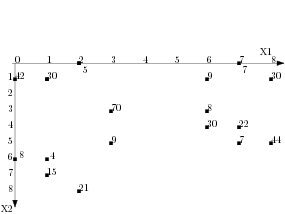
\includegraphics[width=0.7\linewidth]{exampleMatrix}
	\caption{A Sparse 2D Array}
	\label{fig:exampleMatrix}
\end{figure}

 \begin{table}[H]
	\caption{Matrix Market Format\label{tab:matrixmarket}}
	\begin{center}
		\begin{tabular}{ccc}
			\hline
			{\textbf{Row Index}} & {\textbf{Column Index}} & {\textbf{Value}}\\
			\hline
			1 & 0 & 42 \\
			1 & 1 & 30\\
			0 & 2 & 5\\
			3 & 3 & 70\\
			5 & 3 & 9\\
			6 & 0 & 8 \\
			6 & 1 & 4 \\
			7 & 1 & 15 \\
			8 & 2 & 21 \\
			5 & 8 & 44\\
			1 & 8 & 30\\
			0 & 7 & 7\\
			1 & 6 & 9\\
			3 & 6 & 8\\
			4 & 7 & 22\\
			4 & 6 & 30\\
			5 & 7 & 7 \\
			\hline
		\end{tabular}
	\end{center}
\end{table}

\subsection{Linked List}
Linked lists  consist of nodes that link the non-zero elements of sparse arrays together using pointers. Each node has four fields. A \textbf{row} field that stores the row index of the non-zero element, a \textbf{column} field that stores the column index of the non-zero element, a \textbf{value} field that holds the value of the non-zero element located at index – <row,column>, and a \textbf{next node} field that indicates the address of the next node. Figure \ref{fig:linkedList} provides the basic architecture for a linked list representation.

 \begin{figure}[H]
	\centering
	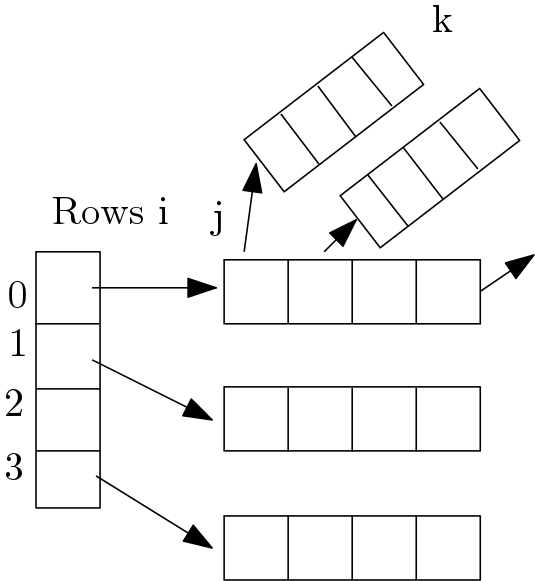
\includegraphics[width=0.3\linewidth]{LinkedList}
	\caption{Linked List Representation}
	\label{fig:linkedList}
\end{figure}

\textbf{Pros}
\begin{compactitem}
	\item Linked lists are fine if all of the data and processing is done in memory.
	\item Linked lists are extendible.
\end{compactitem}

\textbf{Cons}
\begin{compactitem}
	\item Linked lists are inappropriate for large files on the disk memory as linked lists can't be organized on the disk. As data warehousing works with big data the storage schema needs to be stored on the disk. 
\end{compactitem}

\subsection{Compressed Row/Column Storage}

 CRS representation makes use of three one-dimensional arrays to represent sparse 2D arrays. The \textbf{Value} array holds the non-zero elements from the 2D array, the \textbf{Column index} array holds the column indexes of each non-zero element, and the \textbf{Row pointer} array holds the offset value that starts a row \cite{wang:2014sar}.
 
 Using the example data given in Table \ref{tab:matrixmarket} and Figure \ref{fig:exampleMatrix} we give the CRS representation as shown in Table \ref{tab:compressed}.
 
  \begin{table}[H]
 	\caption{Compressed Row Storage Representation\label{tab:compressed}}
 	\begin{center}
 		\begin{tabular}{lllllllllllll}
 			\hline
 			{\textbf{Offset}} & 0 & 1 & 2 & 3 & 4 & 5 & 6 & ...& 14 & 15 & 16 & 17\\
 			\hline
 			{\textbf{Value}} & 5 & 7 & 42 & 30 & 9 & 30 & 70 & ...& 4 & 15 & 21 & 17 \\
 			{\textbf{Column index}} & 2 & 7 & 0 & 1 & 6 & 8 & 3 & ... & 1 & 1 & 2 & 17\\
 			{\textbf{Row Pointer}} & 0 & 2 & 6 & 8 & 10 & 12 & 13 & 15 & 16 & 17 & & \\
 			\hline
 		\end{tabular}
 	\end{center}
 \end{table}

\textbf{Pros}
\begin{compactitem}
	\item CRS and CCS have a wide usage - mainly with 2D arrays and image processing.
\end{compactitem}

\textbf{Cons}
\begin{compactitem}
	\item CRS and CCS are not appropriate representations of data stored on disk.
	\item CRS and CCS are not extendible - they require reorganising the entire array representation with the new additions by extending the bounds. Thus CRS and CCS are not appropriate in a dynamic environment when changes are happening rapidly.
	\item CRS and CCS representations are not appropriate for large arrays.
\end{compactitem}

\subsection{Bit Encoded Sparse Storage}
BESS uses a concatenation of the bit encoded representations of the indexes to generate a Bit Encoded Index (BEI). To improve storage for this method, a level of partitioning known as chunking is used. If $h_i, 0\leq i < k$ is the size of the chunk in each dimension, the number of chunks is $\prod_{i=0}^{k-1}[\frac{n_i}{h_i}]$. The storage required is $(\prod_{i=0}^{k-1}[\frac{n_i}{h_i}])*((c+ [\frac{\sum_{i=0}^{k-1}[\log h_i]}{wordsize}])N_{chunk})$. Only chunks that contain non-zero elements are stored.

For the example provided in Figure \ref{fig:exampleMatrix} if we were to divide the 2D array into 3x3 chunks we would get Figure \ref{fig:chunk} where the chunks breaks and discarded chunks are shown in blue.

 \begin{figure}[H]
	\centering
	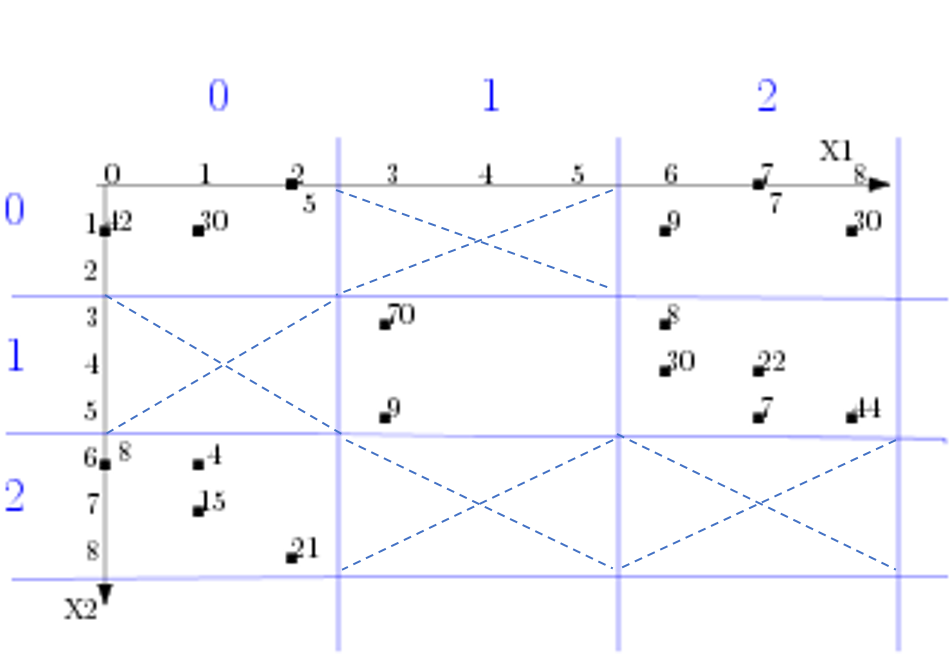
\includegraphics[width=0.7\linewidth]{chunked}
	\caption{BESS Chunking}
	\label{fig:chunk}
\end{figure}

The content from a non-empty chunk is stored as either a dense array or by using a sparse array method depending on the sparsity of the chunk.

\subsection{Comparisons of the Different Representations}

CRS and CCS are both only used for 2D arrays. In the work of Goil et al. \cite{goil:bess} it is clear that BESS out performs Offset-Value pair. In the work of Wang \cite{wang:2014sar} it is evident that although PTCS has a better storage ratio and xCRS/xCCS and BxCRS have faster element retrieval times, BESS has a faster construction time and a faster multi-dimensional aggregation time than all of the other storage schemes. 

BESS is a very simple and efficient multi-dimensional sparse array representation as it maps a multi-dimensional sparse array space to a one-dimensional array space, resulting in a bit encoded key index \cite{wang:2014sar}. A multi-dimensional sparse array data model using a BESS array representation scheme as well as a model using a CRS representation scheme will be analysed.

%%%%%%%%%%%%%%%%%%%%%%%%%%%%%%%%%%%%%%%%%%%%%%%%%%%%%%%%%%%%%%%%%%%%%%%%%%%%%%%%
\section{Extendible Multi-Dimensional Sparse Array Representation}

 By making use of chunking techniques on a BESS array representation scheme as well as a CRS array representation scheme. The proposed extendibility model can increase the dimensionality of the storage scheme by either increasing the density of the array or increasing the dimension of the indices or bounds of the array. When increasing a sparse array by density, the bounds and structure remain the same, new elements are slotted into a chunk where there was a free space. Extendibility of the bounds of the array is done by appending new chunks to the array. The two different extendibility techniques are displayed in red in Figure \ref{fig:examplemethod}.
 
  \begin{figure}[H]
 	\centering
 	\includegraphics[width=0.7\linewidth]{methodExampleCrossed2}
 	\caption{A Sparse 2D Array}
 	\label{fig:examplemethod}
 \end{figure}

\subsection{Multidimensional Sparse Array Blocks}
 In order to organise the chunks easily for reading and writing, a linear index of the array needs to be generated. Mapping for conventional arrays is done using row major order or column major order \cite{otoo:2013:ced}. Using column major order we have 
 \begin{equation}
 	\begin{split}
 		<i,j,k> & = C_0 C_1 C_2 \\
 		<i_0,j_0,k_0> = I & = i_0C_0 + j_0C_1 + k_0C_2
 	\end{split}
 \end{equation}
 where:
 \begin{align*}
 	C_0 & = X_1 \cdot X_2,\\
 	 C_1 & = X_2, \\
 	 C_2 & = 1
 \end{align*}
 
 An in memory index needs to be built into the blocks. As the indexing needs to be done in memory, multi-branching is not optimal, thus we focus on two way branching. Two important two way branches are the binary tree, and the PATRICIA Trie. Binary search trees are not balanced and can be skewed wasting storage space. PATRICIA stands for Practical Algorithm to Retrieve Information Coded In Alphanumeric \cite{morrison1968}. In PATRICIA Tries the skewness is compressed as it only compares bits that change the path and skips levels that are the same. If the chunk index values are stored and organised in a PATRICIA Trie we will avoid heavy sided trees and allow easy access to reading and writing of the array.
 
 \subsubsection{PATRICIA Trie representation of Blocks}
 Using the example in Figure \ref{fig:examplemethod} by labelling each chunk as A, B, C, D and E respectively and assigning their 2-bit row and 2-bit column indexing we obtain the bit indexing of the BESS chunks as shown in Table \ref{tab:index}. From this representation the PATRICIA Trie in Knuth representation is given in Figure \ref{fig:knuth}.
 
\begin{table}[H]
	\caption{Bit Indexing of BESS Chunks}\label{tab:index}
	\begin{center}
		\begin{tabular}{lll}
			\hline
			 \textbf{Linear Position} & \textbf{Bits} & \textbf{Chunk} \\
			\hline
			0 & 0000 & A \\
			2 & 0010 & B \\
			4 & 0100 & C \\
			5 & 0101 & D \\
			6 & 0110 & E \\
			\hline
		\end{tabular}
	\end{center}
\end{table}
 
 \begin{figure}[H]
 	\centering
 	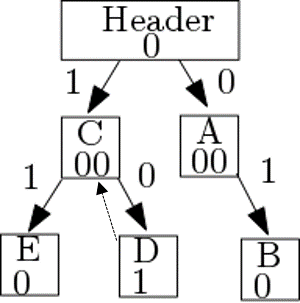
\includegraphics[width=0.25\linewidth]{knuth1}
 	\caption{Knuth representation of PATRICIA Trie indexing for the example in Figure \ref{fig:examplemethod}}
 	\label{fig:knuth}
 \end{figure}
 
 \section{Methodology for Accessing an Element from a Compressed Sparse Array}
 Suppose we have the compressed sparse array given in Figure \ref{fig:examplemethod} and we wish to find element 20 at position $<4,6>$. We will need to take the floor of the row and column indexes divided by the bounds of the matrix. I.e. we have $ \lfloor\frac{4}{3}\rfloor = 1$ and $\lfloor\frac{6}{3}\rfloor = 2$. Thus the block index is located at $<1,2>$ which has a linear address of $5$. We then use the PATRICIA Trie to locate the block. Once the block has been located, we use row major order to locate the element in the linear matrix within the block.
 
 \section{Project methodology}
 A sparse Big Data database will need to be sourced and stored. A BESS compression method as well as a CRS compression method will be applied to the database.
  
 The two algorithms for extension by appending and by inserting will need to be developed and implemented in software in order to determine which algorithm performs better. To assess the performance of the extendible multi-dimensional models, a measure of the storage efficiency and order of retrieval of queries shall be conducted using basic construction, low level retrieval and partial match query array operations.
 
 The two algorithms will be tested on a 2D array (both CRS and BESS), a 3D array(only BESS) and a 4D array(Only BESS) to asses their limitations on different dimensionalities.
 
 Figure \ref{fig:proposedmethod} shows the main steps in the proposed methodology of the project.
 
 \begin{figure}[H]
 	\centering
 	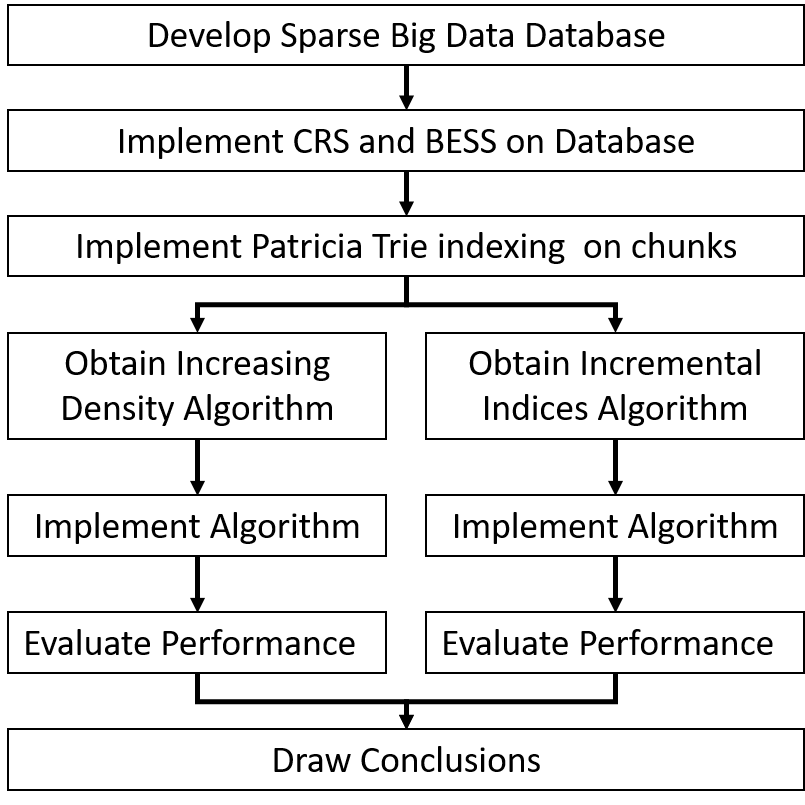
\includegraphics[width=0.7\linewidth]{proposedMethod2}
 	\caption{Proposed Methodology}
 	\label{fig:proposedmethod}
 \end{figure}
 
This representation can then be used in data warehousing where items are increased, stores can be acquired in new locations and new time frames can be added.

%!TEX root = main-doc.tex
%
% File: experimentalsetup.tex
%
% Date: ? 
%
% Description:
%   
%
%
\chapter{Experimental Setup} \label{chap:experimentalsetup}
\vspace{-1cm}
%\summary{This chapter details the computational environment and the experimental data in order to allow for independent reproducibility and confirmation of the conducted experiments.}

%%%%%%%%%%%%%%%%%%%%%%%%%%%%%%%%%%%%%%%%%%%%%%%%%%%%%%%%%%%%%%%%%%%%%%%%%%%%%%%%
%\vspace{-1cm}
\section{Computational Environment}

%%%%%%%%%%%%%%%%%%%%%%%%%%%%%%%%%%%%%%%%%%%%%%%%%%%%%%%%%%%%%%%%%%%%%%%%%%%%%%%%
%\subsection{Experimental Computational Model and Software Environment}
The experiments will be run on a laptop with an Intel(R) Core(TM) i5-2450 multi-core processor at 2.50~GHz and 4GB of memory running Ubuntu 64-bit Linux 16.04.3 LTS.

The experiments will be implemented in C using GNU Compiler Collection (GCC) 7.2.

%%%%%%%%%%%%%%%%%%%%%%%%%%%%%%%%%%%%%%%%%%%%%%%%%%%%%%%%%%%%%%%%%%%%%%%%%%%%%%%%
%\section{Experimental Data}

%\textbf{NB - Still working on this section}

%%%%%%%%%%%%%%%%%%%%%%%%%%%%%%%%%%%%%%%%%%%%%%%%%%%%%%%%%%%%%%%%%%%%%%%%%%%%%%%%
%\section{Software Engineering Practice}

%\textbf{NB - Still working on this section}
%!TEX root = main-doc.tex
%
% File: preliminaryresults.tex
%
% Date: ? 
%
% Description:
%   The background is given to ...
%
%
\chapter{Preliminary Results} \label{chap:preliminaryresults}
\vspace{-1cm}
%\summary{This chapter provides an outline of any preliminary experiments that have been conducted on the extendibility of multidimensional sparse arrays.}

%%%%%%%%%%%%%%%%%%%%%%%%%%%%%%%%%%%%%%%%%%%%%%%%%%%%%%%%%%%%%%%%%%%%%%%%%%%%%%%%
\section{Investigations on Pre-existing Technologies}
Some preliminary investigations have been conducted on pre-existing Big Data formats and pre-existing data analysis platforms. A quick overview of the TileDB storage manager shows that the storage manager only caters for 2D sparse arrays and does not cater for higher dimensions. TileDB inserts new data into sparse arrays by storing the new data in previously empty cells \cite{tiledb:tm101}. A look at two data analysis platforms, Weka and RapidMiner, show how pre-existing technologies cater for MOLAP operations, however the platforms do not allow for any extendibility of the actual datasets they are operating on.

%%%%%%%%%%%%%%%%%%%%%%%%%%%%%%%%%%%%%%%%%%%%%%%%%%%%%%%%%%%%%%%%%%%%%%%%%%%%%%%%
\section{XSAS Implementation in C}
Some coding has been conducted in C making use of the GNU Scientific Library. The example matrix given in Figure \ref{fig:exampleMatrix} was stored using CRS. The program is currently being extended to store the matrix using BESS. Once the BESS algorithm has been implemented the code will be extended to incorporate PATRICIA Trie indexing. Upon completion of the PATRICIA Trie indexing the density extendibility and the bounds extendibility algorithms will be implemented and their performances analysed.
%!TEX root = main-doc.tex
%
% File: futurework.tex
%
% Date: ? 
%
% Description:
%   The background is given to ...
%
%
\chapter{Future Work} \label{chap:futurework}

\summary{Give chapter summary}

%%%%%%%%%%%%%%%%%%%%%%%%%%%%%%%%%%%%%%%%%%%%%%%%%%%%%%%%%%%%%%%%%%%%%%%%%%%%%%%%
%\section{Data Warehousing}
%%!TEX root = main-doc.tex
%
% File: validationofresults.tex
%
% Date: ? 
%
% Description:
%   The background is given to ...
%
%
\chapter{Validation of Results} \label{chap:validationofresults}
\vspace{-1cm}
%\summary{Give chapter summary}

%%%%%%%%%%%%%%%%%%%%%%%%%%%%%%%%%%%%%%%%%%%%%%%%%%%%%%%%%%%%%%%%%%%%%%%%%%%%%%%%
%\section{Data Warehousing}
In order to test the performance and efficiency of the proposed solution, several tests will be run. Experiments similar to the ones done in \cite{otoo:2013:ced}, \cite{pedereira:2015:cas}, \cite{otoo:2016:msa} and \cite{goil:bess} and will be done where three datasets of different sizes, three datasets of different dimensions (2D,3D and 4D) and three datasets of different sparsity levels (i.e. 80\%, 90\% and 95\%) will be stored in the XSAS representation (i.e. six different datasets). Three different queries will be run and timed on the datasets, these queries will be run three times each in order to ensure that an accurate average measurement has been taken. An assessment of the storage utilization (in percentage) will be done on the arrays. A further investigation will be conducted on 2D arrays comparing the XSAS representation with BESS and the XSAS representation with CRS.
%!TEX root = main-doc.tex
%
% File: riskmanagement.tex
%
% Date: ? 
%
% Description:
%   The background is given to ...
%
%
\chapter{Risk Management} \label{chap:riskmanagement}
%\vspace{-1cm}
%\summary{Give chapter summary}

%%%%%%%%%%%%%%%%%%%%%%%%%%%%%%%%%%%%%%%%%%%%%%%%%%%%%%%%%%%%%%%%%%%%%%%%%%%%%%%%
%\section{Data Warehousing}
%!TEX root = main-doc.tex
%
% File: schedule.tex
%
% Date: ? 
%
% Description:
%   The background is given to ...
%
%
\chapter{Schedule and Time-Line for Completion} \label{chap:schedule}

\summary{This chapter details the research tasks and their proposed date of completion.}

%%%%%%%%%%%%%%%%%%%%%%%%%%%%%%%%%%%%%%%%%%%%%%%%%%%%%%%%%%%%%%%%%%%%%%%%%%%%%%%%
\section{Estimated Task Completion Time-Line}

\begin{tabular}{|l|l|}
	\hline 
	\textbf{Task Description} & \textbf{Deadline} \\ 
	\hline 
	 Begin Research Project & January 2017\\
	 Literature Review of Data Warehousing & March 2017\\
	 Literature Review of Sparse Array Representation & May 2017\\
	 Literature Review of Dynamic Dense Array Representation & July 2017\\
	 Documentation of the Methodology & September 2017\\
	 Submit Research Proposal for Approval & October 2017\\
	 Visual Presentation of the Research Proposal & October 2017 \\
	 Develop and Implement Storage and Chunking Techniques & December 2017\\
	 Develop Dynamic Expansion Algorithms & February 2018\\
	 Evaluate Performance and Analyse Results & April 2018\\
	 Submit Research Dissertation for Approval & April 2018\\
	\hline 
\end{tabular} 
%!TEX root = main-doc.tex
%
% File: summary.tex
%
% Date: ? 
%
% Description:
%   The background is given to ...
%
%
\chapter{Summary} \label{chap:summary}
%\vspace{-1cm}
%\summary{Give chapter summary}

%%%%%%%%%%%%%%%%%%%%%%%%%%%%%%%%%%%%%%%%%%%%%%%%%%%%%%%%%%%%%%%%%%%%%%%%%%%%%%%%
%\section{Data Warehousing}
% \include{conclusion}

%%%%%%%%%%%%%%%%%%%%%%%%%%%%%%%%%%%%%%%%%%%%%%%%%%%%%%%%%%%%%%%%%%%%%%%%%%%%%%%

\newpage

%%%
% Automatically balance the output of the last page
%\balance
%%%

%%%%%%%%%%%%%%%%%%%%%%%%%%%%%%%%%%%%%%%%%%%%%%%%%%%%%%%%%%%%%%%%%%%%%%%%%%%%%%%
%
% References: .bib files, followed by bibliography style
%\nocite{*}
\bibliographystyle{witseie}
%\bibliographystyle{IEEEbib}
\bibliography{sample}

% Appendices
\appendix
\renewcommand{\chaptermark}[1]{\markboth{\appendixname\ \thechapter\ --- #1}{}}

% \include{appendix-1}
% \include{appendix-2}

\end{document}

" vim: ts=4
" vim: tw=78
" vim: autoindent
" vim: shiftwidth=4
